% !TeX spellcheck = es_MX
\documentclass[12pt, a4paper, titlepage]{article}
\usepackage[spanish]{babel}
\usepackage[utf8]{inputenc}
\usepackage[linesnumbered,lined,boxed,commentsnumbered]{algorithm2e}
\usepackage{enumitem,kantlipsum}
\usepackage{array}
\usepackage{placeins}
% Códigos y codificación para caracteres en español
\usepackage{listings}
\usepackage{color}
\lstset{literate=
	{á}{{\'a}}1 {é}{{\'e}}1 {í}{{\'i}}1 {ó}{{\'o}}1 {ú}{{\'u}}1
	{Á}{{\'A}}1 {É}{{\'E}}1 {Í}{{\'I}}1 {Ó}{{\'O}}1 {Ú}{{\'U}}1
	{à}{{\`a}}1 {è}{{\`e}}1 {ì}{{\`i}}1 {ò}{{\`o}}1 {ù}{{\`u}}1
	{À}{{\`A}}1 {È}{{\'E}}1 {Ì}{{\`I}}1 {Ò}{{\`O}}1 {Ù}{{\`U}}1
	{ä}{{\"a}}1 {ë}{{\"e}}1 {ï}{{\"i}}1 {ö}{{\"o}}1 {ü}{{\"u}}1
	{Ä}{{\"A}}1 {Ë}{{\"E}}1 {Ï}{{\"I}}1 {Ö}{{\"O}}1 {Ü}{{\"U}}1
	{â}{{\^a}}1 {ê}{{\^e}}1 {î}{{\^i}}1 {ô}{{\^o}}1 {û}{{\^u}}1
	{Â}{{\^A}}1 {Ê}{{\^E}}1 {Î}{{\^I}}1 {Ô}{{\^O}}1 {Û}{{\^U}}1
	{œ}{{\oe}}1 {Œ}{{\OE}}1 {æ}{{\ae}}1 {Æ}{{\AE}}1 {ß}{{\ss}}1
	{ű}{{\H{u}}}1 {Ű}{{\H{U}}}1 {ő}{{\H{o}}}1 {Ő}{{\H{O}}}1
	{ç}{{\c c}}1 {Ç}{{\c C}}1 {ø}{{\o}}1 {å}{{\r a}}1 {Å}{{\r A}}1
	{€}{{\EUR}}1 {£}{{\pounds}}1
}

%%Appendix
\usepackage[toc,page]{appendix}

%%otros
\usepackage{float}
\usepackage{subfig}
\usepackage{comment}

% http://ctan.org/pkg/booktabs
\usepackage{booktabs}
\newcommand{\tabitem}{~~\llap{\textbullet}~~}

%%Imágenes
\usepackage{graphicx}

%%Colores de texto 
\usepackage{xcolor}
\usepackage{colortbl}

%%Links
\usepackage[hidelinks]{hyperref}

%%Comentarios
\usepackage{verbatim}

%%PARA IMÁGENES EN LÍNEA
%\usepackage[english]{babel}

\usepackage{pdfpages}

%------------------------------------------------ESTABLECER COLORES------------------------------------------------%

\definecolor{guindapoli}{RGB}{102, 0, 51}
\definecolor{azulescom}{RGB}{0, 0, 102}
\definecolor{azulclaro}{RGB}{222, 232, 255}
\definecolor{azulfuerte}{RGB}{60, 150, 250}

%------------------------------------------------FIN DE COLORES------------------------------------------------%


\begin{document}
	%%PARA QUE DETECTE HASTA SUBSUBSECTION
	\setcounter{secnumdepth}{3}
	
	%%%%%%%%%%%%%%%%%%%%%%%%%%%%%%%%%%%%%%%%%%%%%%%%%%%%%%%%%
	%                                                       																																		  %
	%                                                      																																	  		  %
	%              																	PORTADA  																				  			 %
	%                                                      																																			  %
	%                                                      																																			  %
	%%%%%%%%%%%%%%%%%%%%%%%%%%%%%%%%%%%%%%%%%%%%%%%%%%%%%%%%%
	\begin{titlepage}	
		
		\newcommand{\HRule}{\rule{\linewidth}{0.5mm}}									%%%\left
		%%%
		\begin{minipage}{0.48\textwidth} \begin{flushleft}
				
\includegraphics[scale = 0.10]{Imagenes/Logos/logoescom.png}
		\end{flushleft}\end{minipage}
		\begin{minipage}{0.48\textwidth} \begin{flushright}
				
\includegraphics[scale = 0.55]{Imagenes/Logos/logoipn.png}
		\end{flushright}\end{minipage}
		
		%%%
		\vspace*{.25cm}								%%%
		
		\begin{center}
			
			\begin{LARGE}
				\textcolor{guindapoli}{INSTITUTO POLITÉCNICO NACIONAL}\\
			\end{LARGE}	
			
			\vspace*{0.2in}
			
			\begin{Large}
				\textcolor{azulescom}{ESCUELA SUPERIOR DE CÓMPUTO}\\
			\end{Large}	
		
			\vspace*{0.4in}
			
			\begin{large}
				Manual de Usuario\\
			\end{large}	
			
			\vspace*{0.4in}
			
			\begin{large}
				Trabajo Terminal TT2020-B002\\
			\end{large}
			
			\vspace*{0.2in}
			
			\begin{Large}
				\textbf{Generador de versos musicales en el idioma
					inglés por medio de procesamiento de lenguaje
					natural y redes neuronales}\\
			\end{Large}
						
			\vspace*{0.2in}
			
			\rule{80mm}{.1mm}\\
			\vspace*{0.1in}
			
			\begin{large}
				\begin{center}
					\textbf{Presentan}:\\
					Espinosa de los Monteros Lechuga Jaime Daniel\\
					Nava Romo Edgar Adrián\\
					Salgado Gómez Alfredo Emilio\\
				\end{center}
			\end{large}
			
			\begin{large}
				\textbf{Directores}:\\
				Olga Kolesnikova\\
				Ariel López Rojas\\
			\end{large}
			
		\end{center}
		
	\end{titlepage}
	
	%%%%%%%%%%%%%%%%%%%%%%%%%%%%%%%%%%%%%%%%%%%%%%%%%%%%%%%%%
	%                                                       																																		  %
	%                                                      																																	  		  %
	%              																	 ÍNDICE  																				  			 	  %
	%                                                      																																			  %
	%                                                      																																			  %
	%%%%%%%%%%%%%%%%%%%%%%%%%%%%%%%%%%%%%%%%%%%%%%%%%%%%%%%%%
	% Firma directores
	\newpage
	\section*{Firmas de Directores}
	
	\vfill  % push the rest to the bottom of the page
	\noindent 
	\parbox[b]{0.4\linewidth}{% size of the first signature box
		\strut 
		Firmado por: \\[3cm]% This 2cm is the space for the signature under the names
		\hrule
		Profesor: Ariel López Rojas} 
	\hspace{1cm} % distance between the two signature blocks 
	\parbox[b]{0.4\linewidth}{% ...and the second one
		\strut 
		\\[3cm]% This 2cm is the space for the signature under the names
		\hrule
		Doctora Olga Kolesnikova} 
	\par\vspace{1cm} 
	\newpage
	% Rename Appendice to Anexos
	\renewcommand\appendixpagename{Índice}
	\renewcommand\appendixtocname{Índice}
	\appendixpageoff
	\begin{appendices}
		\renewcommand*\contentsname{{\textcolor{azulescom}{Índice.}}}
		\tableofcontents
		\newpage
		%%índice de figuras
		\renewcommand*\listfigurename{{\textcolor{azulescom}{Índice de figuras.}}}
		\listoffigures
		\newpage
		%%Índice de tablas
		\newpage
	\end{appendices}
	
	\section{Introducción}
	El siguiente manual muestra los pasos a seguir para aprovechar en su mayor capacidad la aplicación web la cual permite al usuario generar letras musicales a partir de ciertos parámetros proporcionados por el usuario. Esto con la finalidad de brindar al usuario una herramienta que le asegure el uso correcto de la aplicación web.
	
	\section{Requerimientos}
	Los requerimientos mínimos para que la aplicación web funcione de manera correcta
	\begin{itemize}
		\item Algún dispositivo con conexión a internet (computadora, celular, tablet)
		\item Algún navegador web
	\end{itemize}

	\section{Acceso a la aplicación web}
	Para poder acceder a la aplicación web es necesario que ingrese a la siguiente dirección web x en la cual, una vez desplegada podrá interactuar con ella, a continuación, se muestra la página de inicio:
	\begin{figure}[H] 
		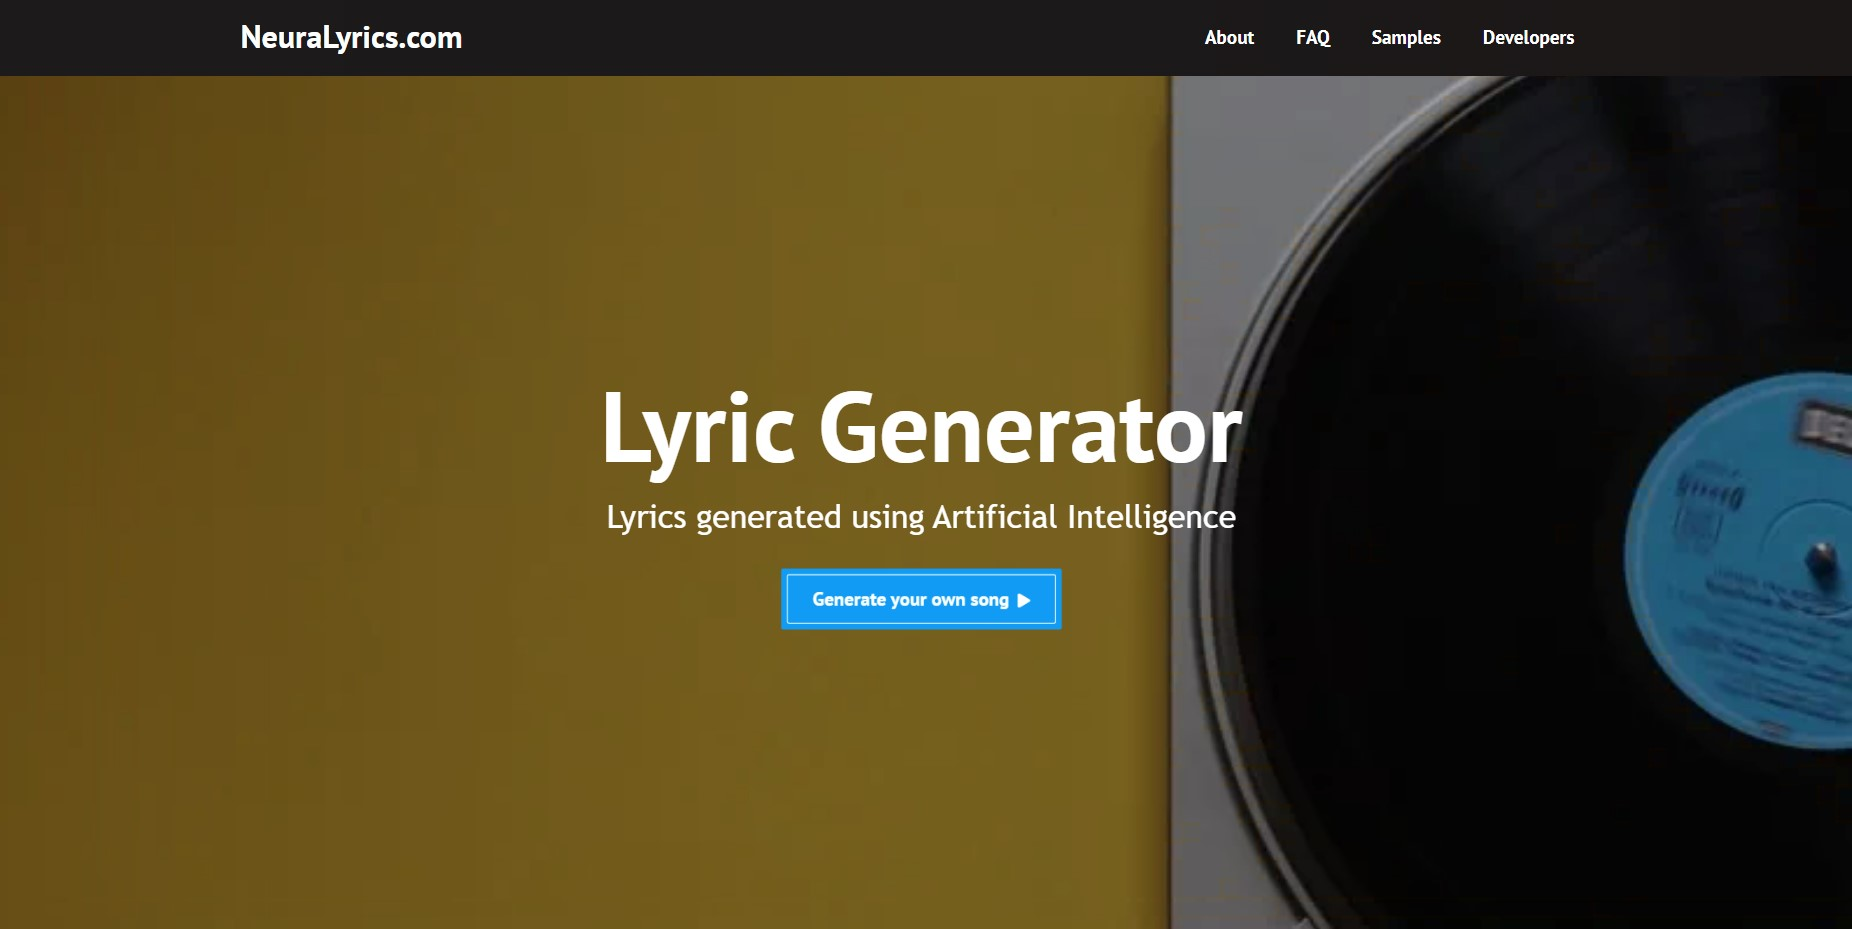
\includegraphics[width=13.5cm]{./Imagenes/Capturas/pprincipal.jpg}
		\centering \caption{Página de inicio de la aplicación web}
	\end{figure}
	Dentro de esta página se mostrará una barra superior en la cual se muestra un menú de opciones que permiten al usuario conocer más sobre la aplicación web, preguntas frecuentes, así como ejemplos de textos generados con anterioridad.\\\\
	En el centro de la página principal se despliega una leyenda seguida de un botón invitando al usuario a generar su propia de letra de canción. Si el usuario hace clic en dicho botón se desplegará el siguiente formulario.
	\begin{figure}[H] 
		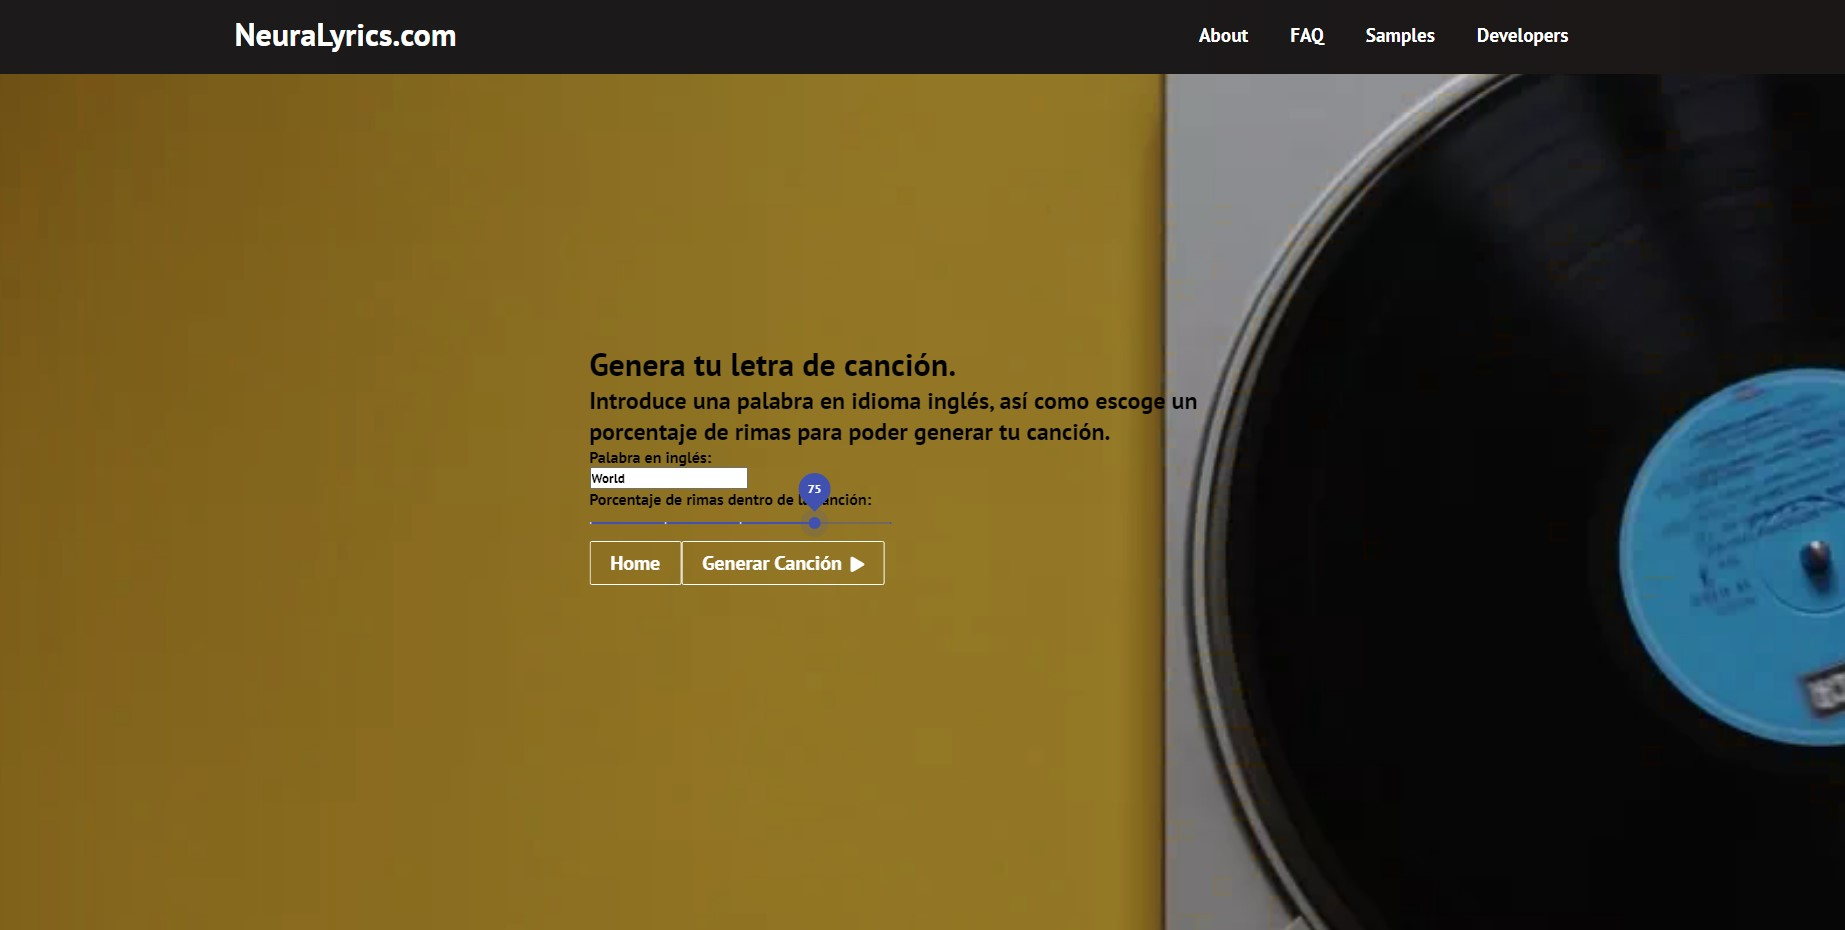
\includegraphics[width=13.5cm]{./Imagenes/Capturas/pformulario.jpg}
		\centering \caption{Formulario de la aplicación web}
	\end{figure}
	Como podemos observar, el formulario pide que el usuario ingrese una palabra en el idioma inglés, así como un porcentaje el cual representa que tanto quiere que la letra de la canción rime, este porcentaje solo admite los siguientes valores (0\%,25\%,50\%,75\%,100\%), esto debido a que es difícil estimar en un texto valores que no son cerrados.\\\\
	Una vez proporcionados los valores por el usuario puede dar clic en el botón de generar canción, lo que provocara que el formulario desaparezca de la pantalla del usuario y muestre un texto indicando que se esta trabajando en generar la letra de su canción y que el usuario tenga paciencia.
	\begin{figure}[H] 
		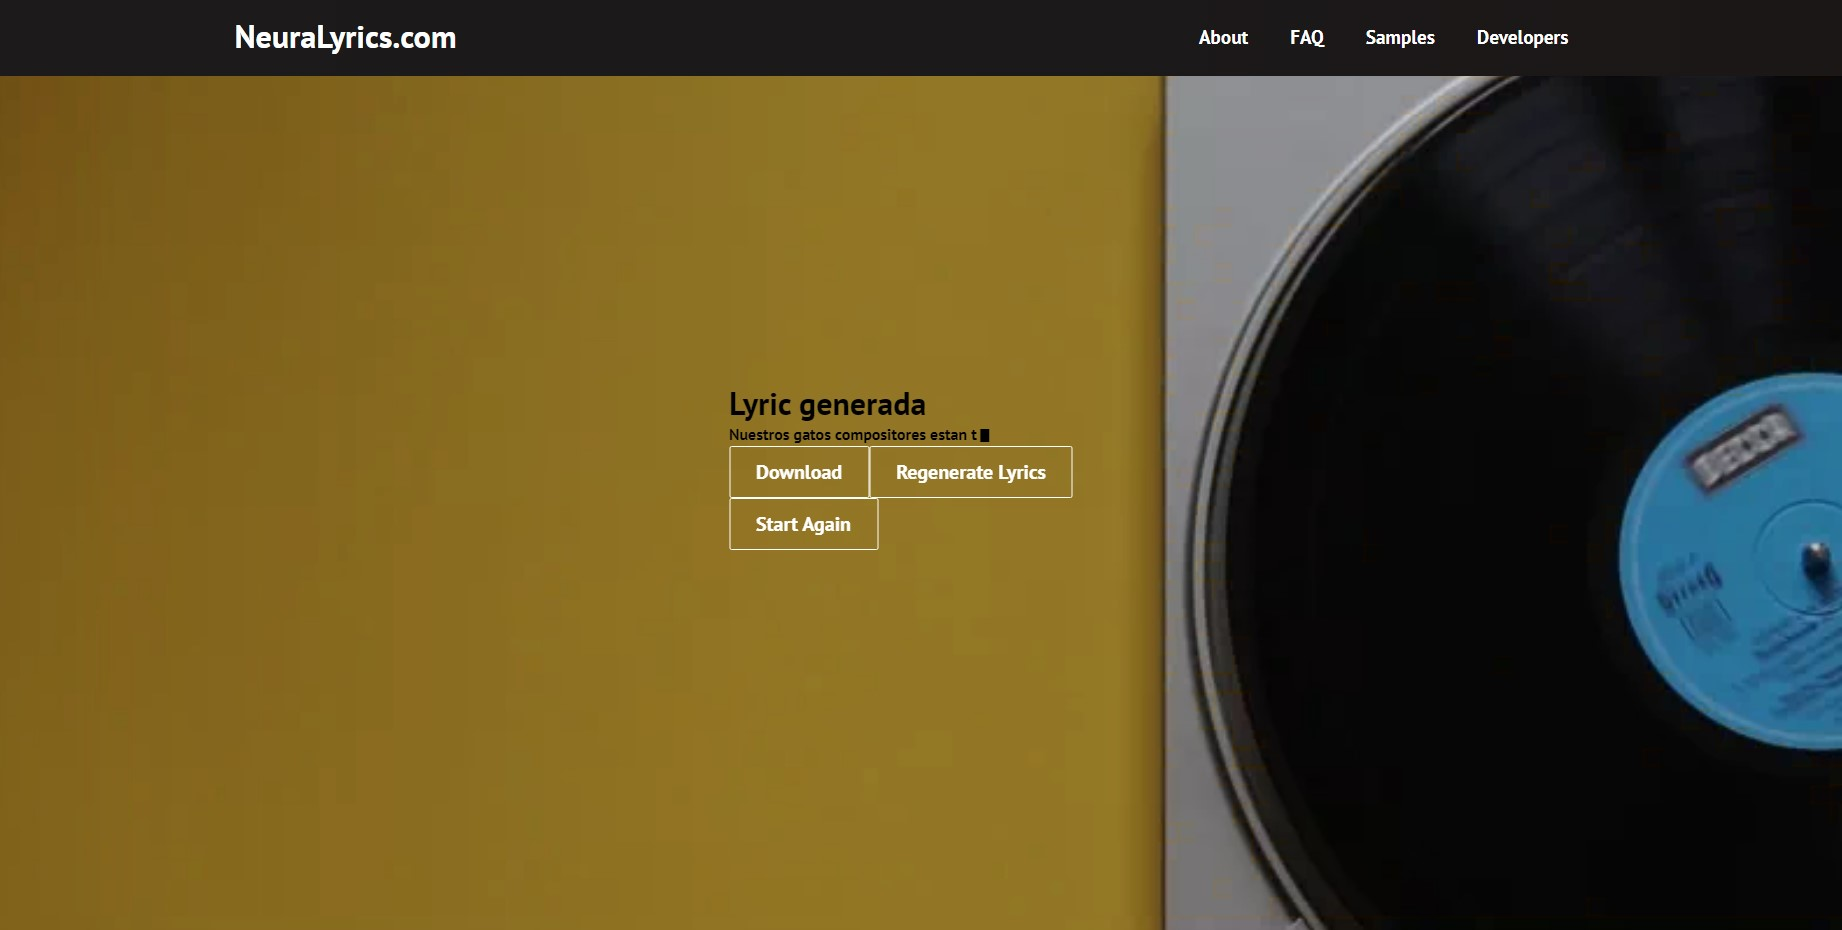
\includegraphics[width=13.5cm]{./Imagenes/Capturas/pcortina.jpg}
		\centering \caption{Cortina de espera}
	\end{figure}
	Este texto se retirará de la pantalla después de unos segundos, mostrando al usuario una ventana en la cual con una animación de tipo máquina de escribir se despliega la letra generada usando los valores proporcionados por el usuario
	\begin{figure}[H] 
		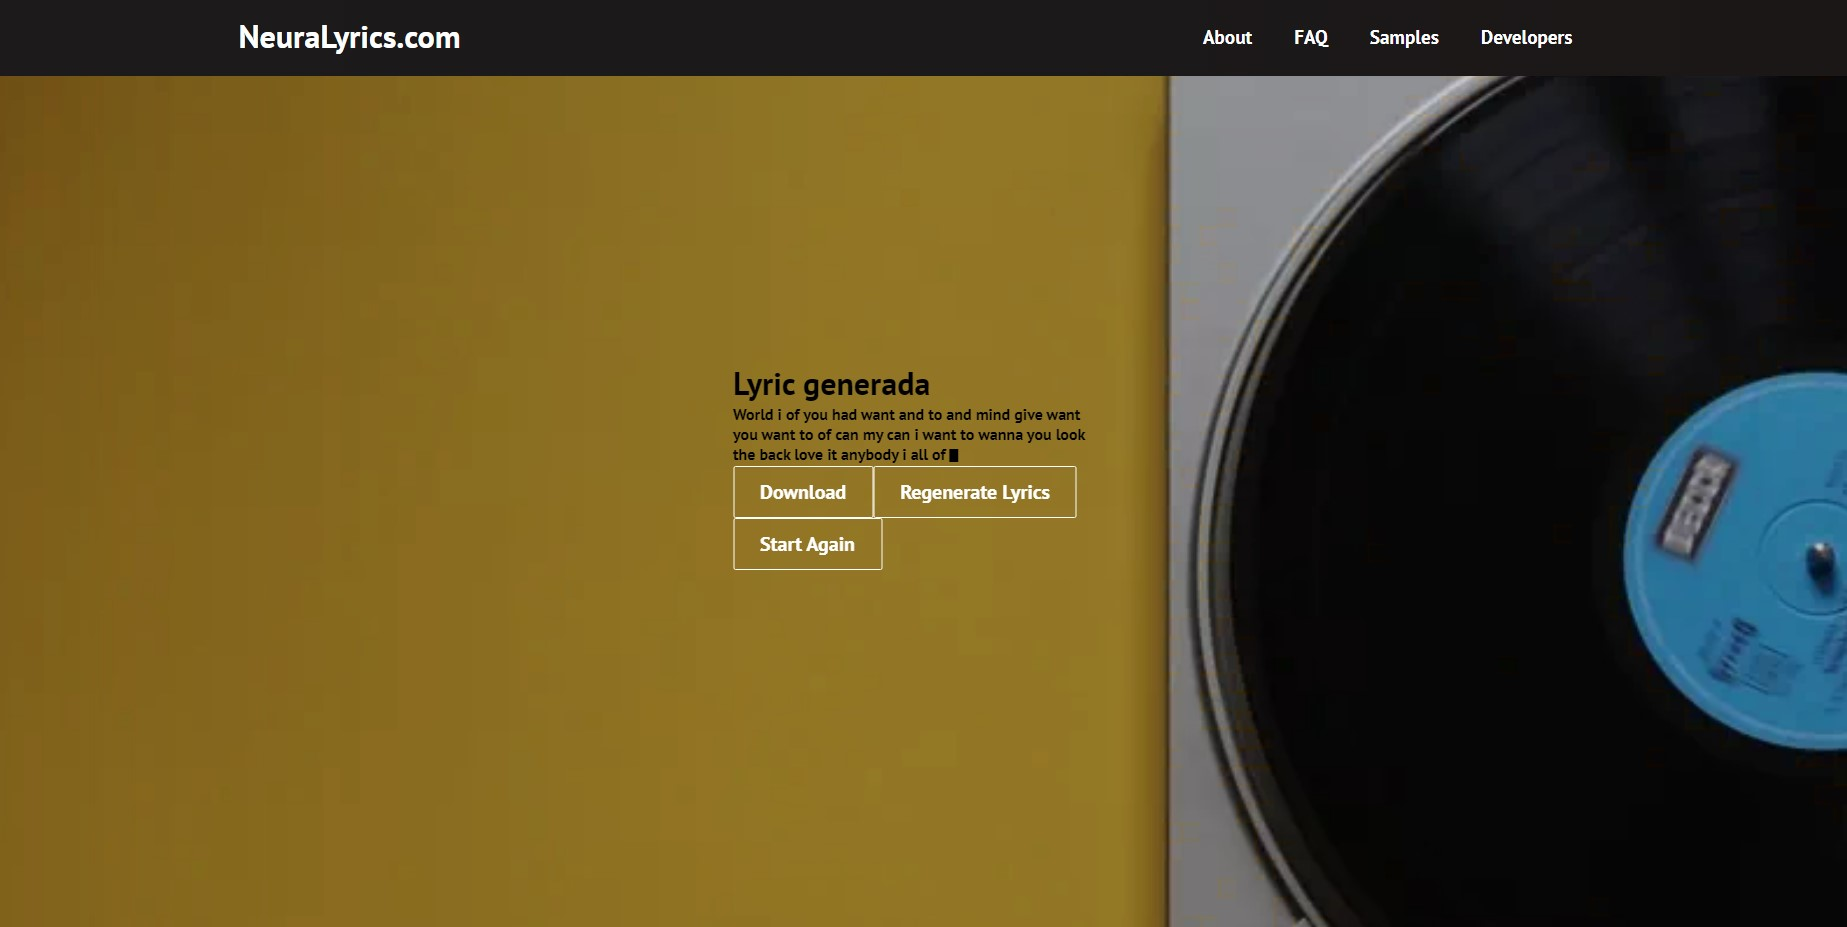
\includegraphics[width=13.5cm]{./Imagenes/Capturas/ptextogenerado.jpg}
		\centering \caption{Página del texto generado}
	\end{figure}
	Como podemos observar en la imagen anterior además del texto generado mostrado en pantalla, brindamos la opción de que el usuario vuelva a generar la letra de la canción utilizando los mismos parámetros que había introducido con anterioridad o si lo desea generarla con unos nuevos.\\\\ 
	Además,se le da la opción al usuario de descargar este texto generado en un archivo de texto, permitiendo así al usuario modificar la letra de la canción generada a su gusto.	
	\begin{figure}[H] 
		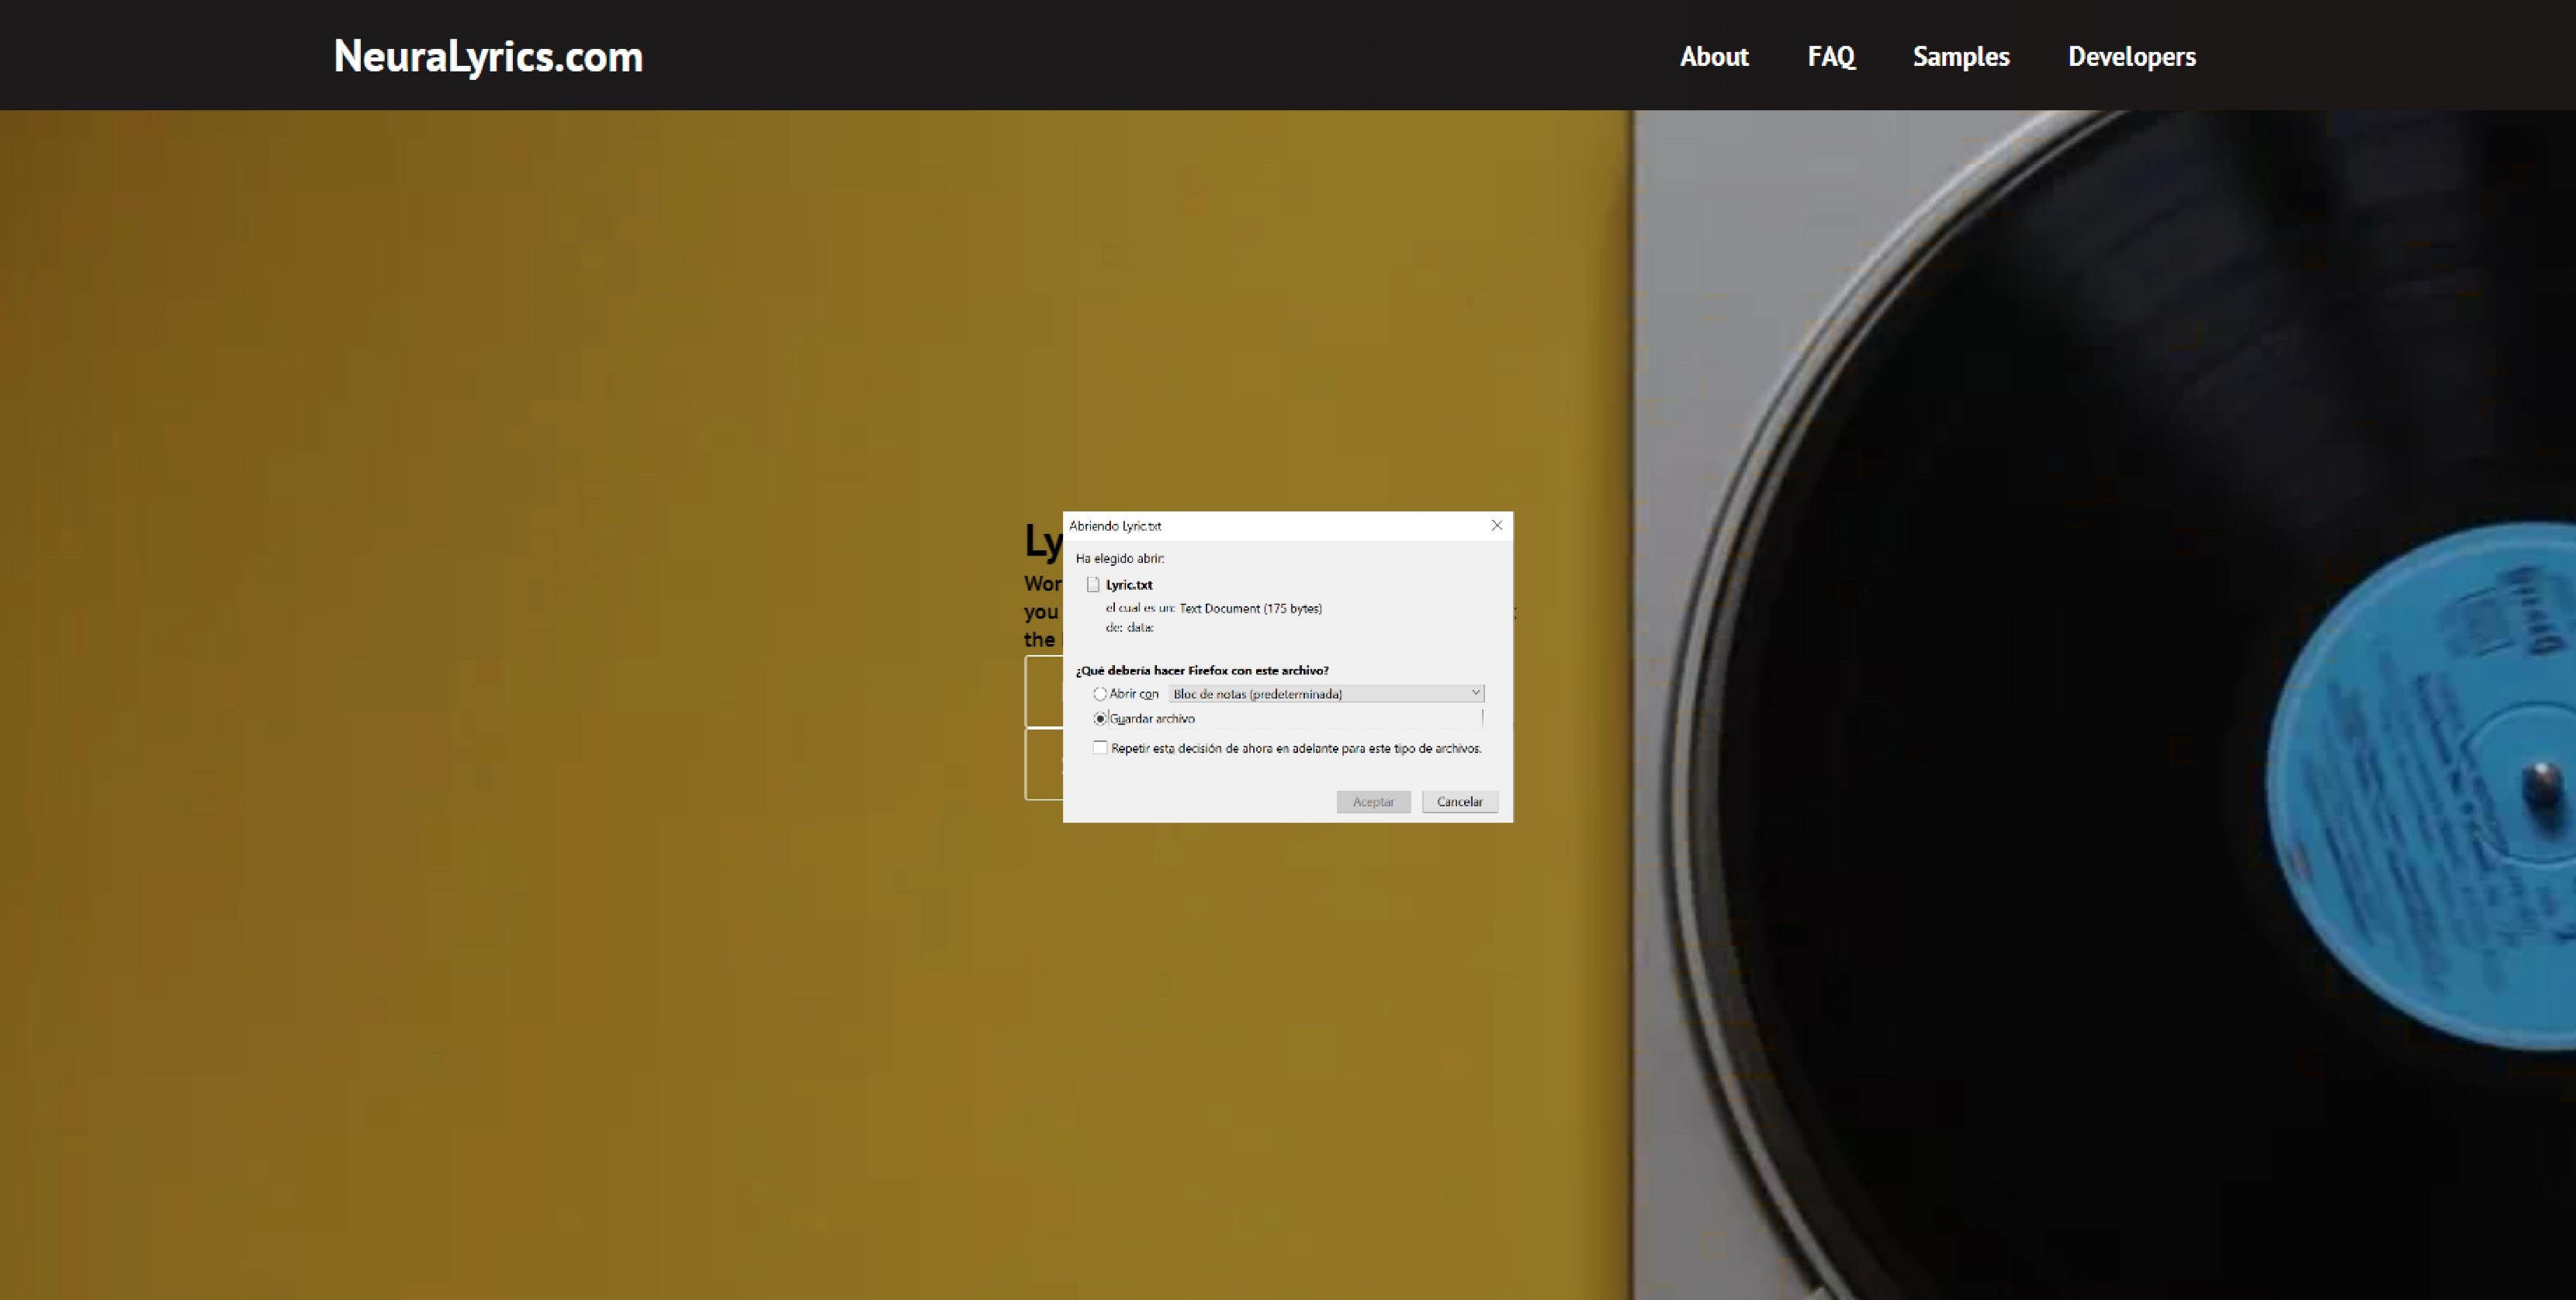
\includegraphics[width=13.5cm]{./Imagenes/Capturas/pdescarga.jpg}
		\centering \caption{Descarga del archivo txt}
	\end{figure}
	\begin{figure}[H] 
	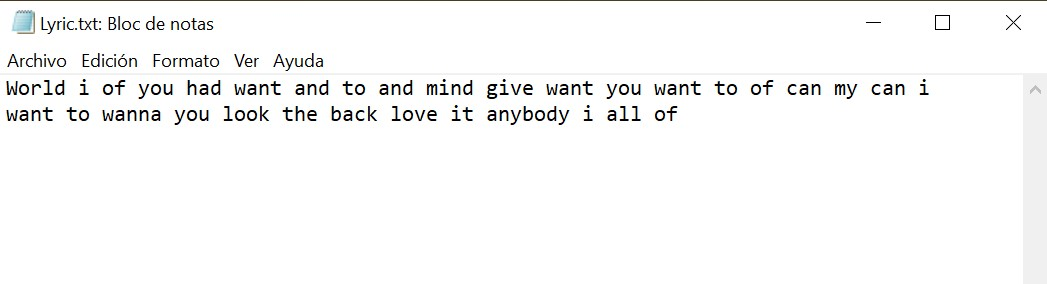
\includegraphics[width=13.5cm]{./Imagenes/Capturas/pvisualizacion.jpg}
	\centering \caption{Visualización del archivo descargado}
	\end{figure}
	Si el usuario accede a la pagina de ejemplos dentro de esta encontrara una tabla la cual indica al usuario la palabra que se utilizó para la generación del texto y un enlace que al momento de darle clic descargara el archivo de texto con el texto generado en esa ocasión.
	\begin{figure}[H] 
		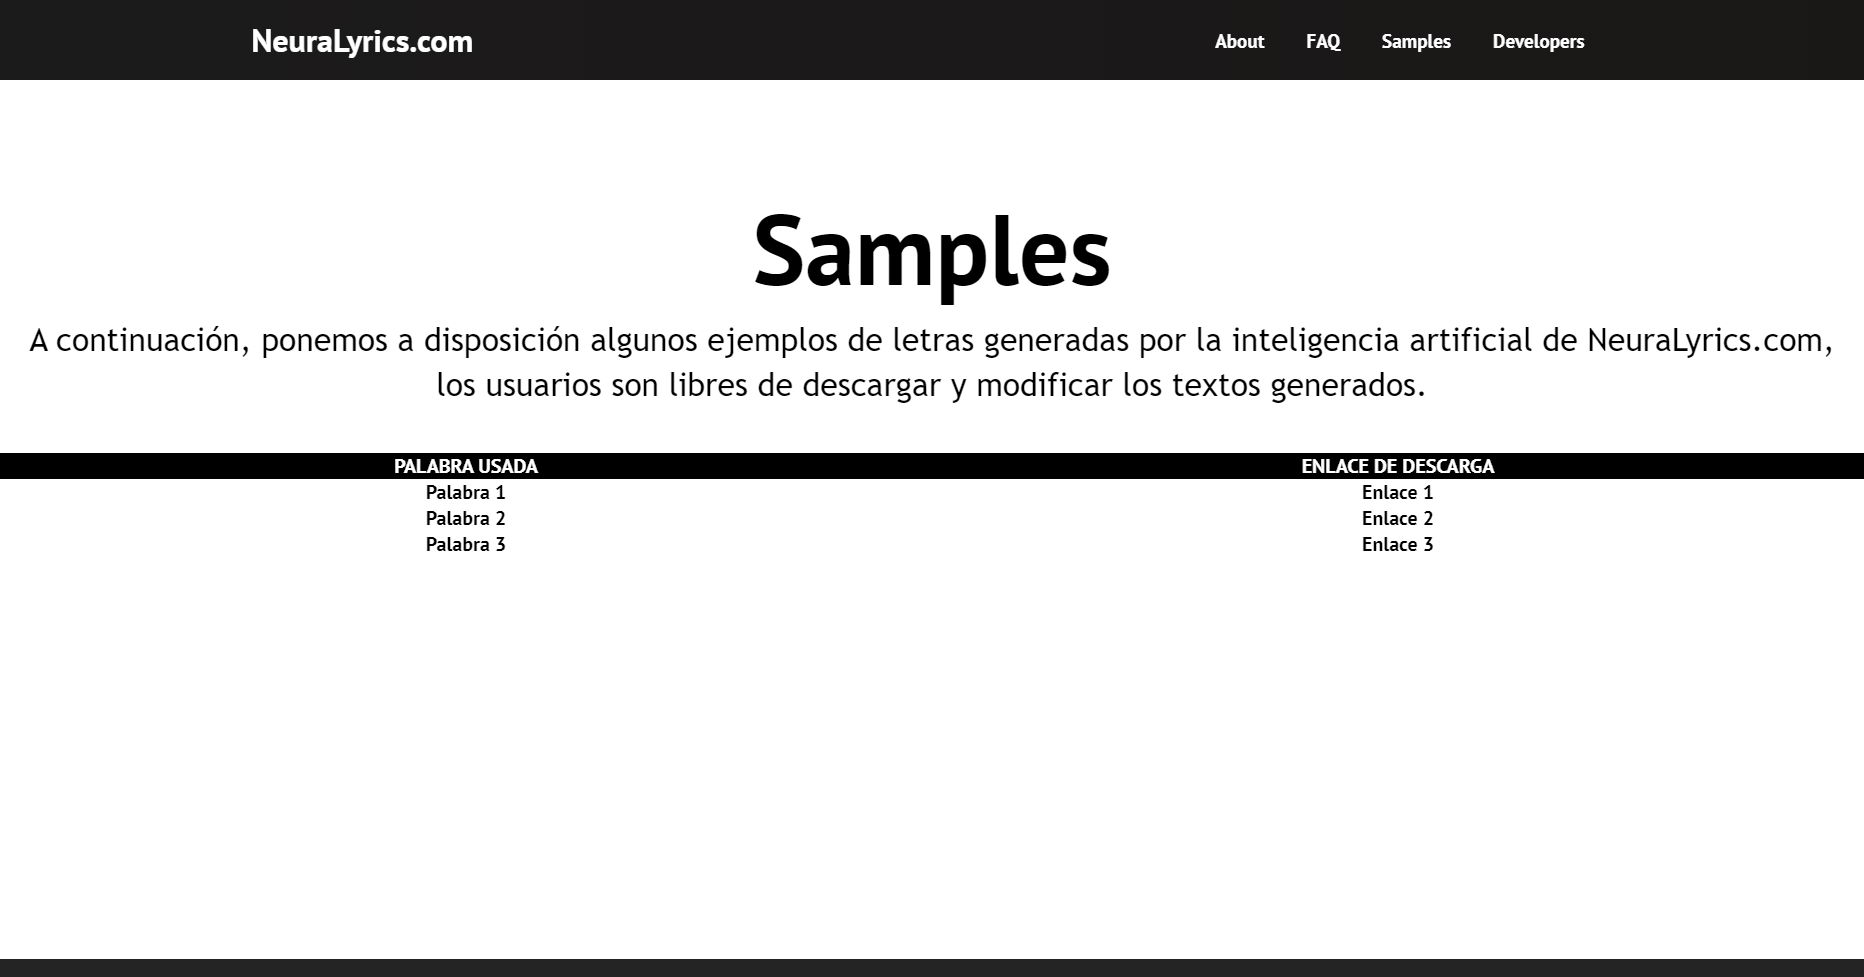
\includegraphics[width=13.5cm]{./Imagenes/Capturas/pejemplos.png}
		\centering \caption{Pagina textos previamente generados}
	\end{figure}
	Si el usuario accede a la pestaña de developers, puede ver como es que funciona a grandes rasgos la parte encargada de la generación de textos, y si el usuario cuneta con ciertos conocimientos en el área de programación puede utilizar esta parte para conectarla y utlizarla en sus propios proyectos.
	\begin{figure}[H] 
		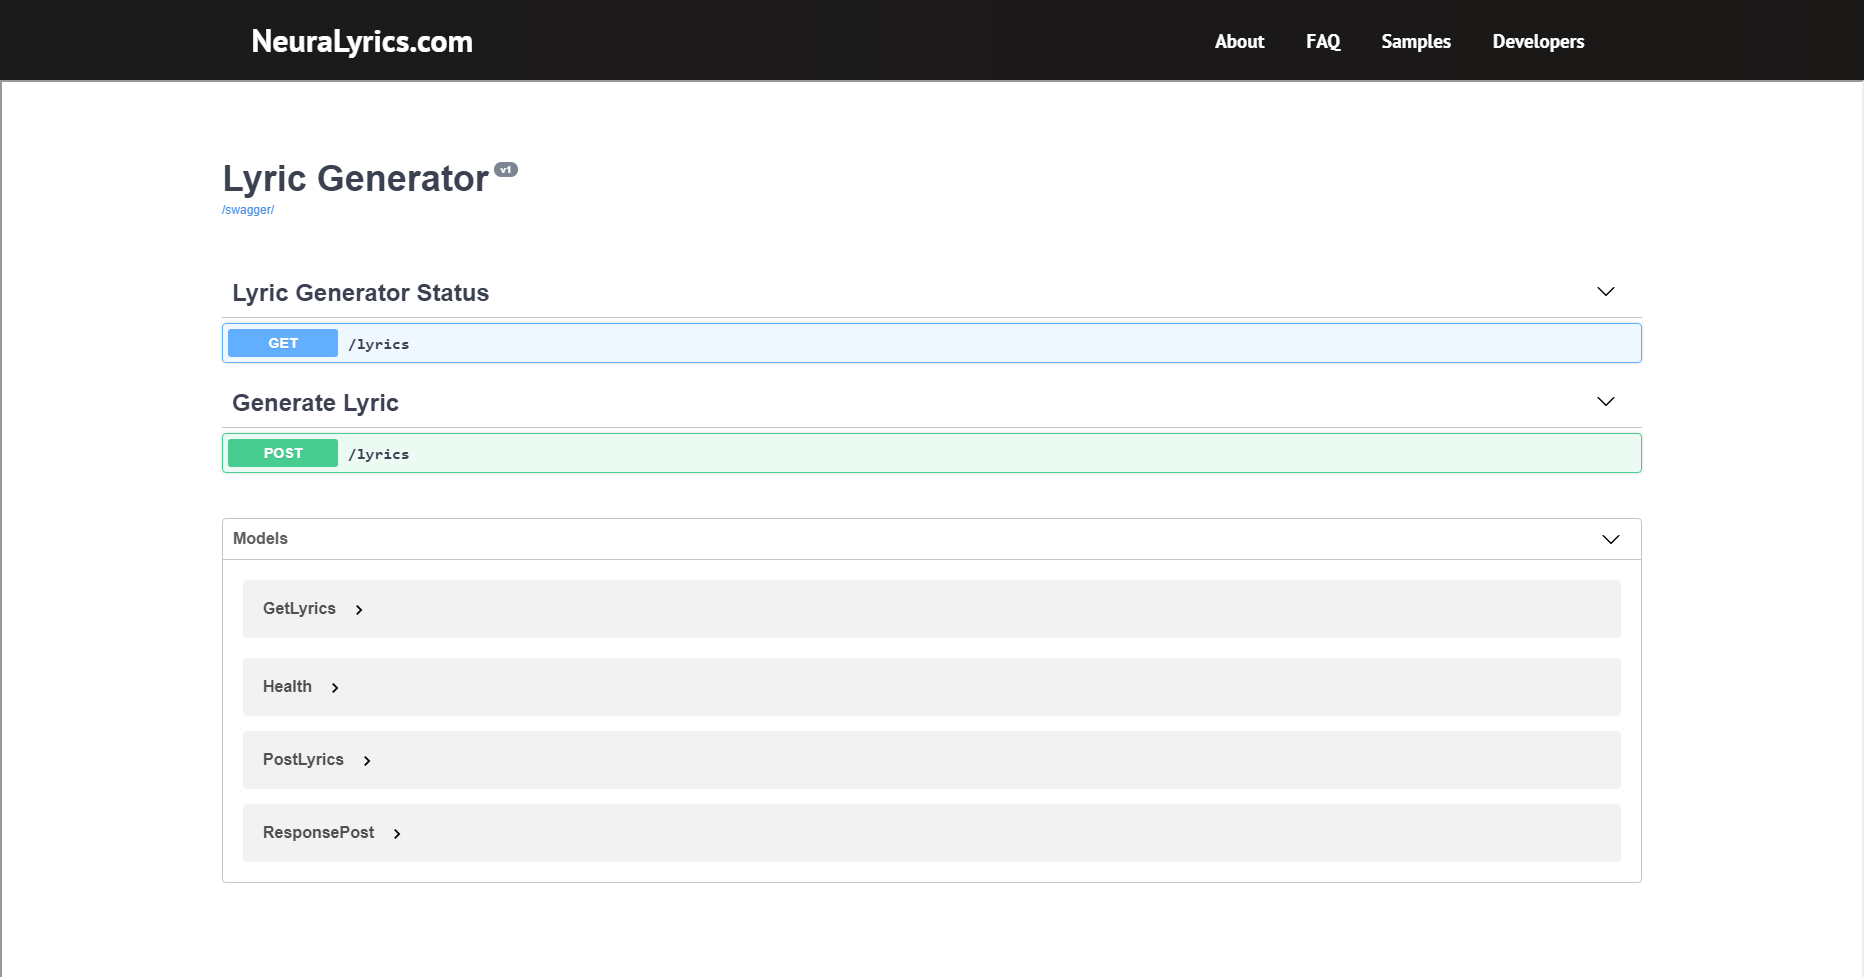
\includegraphics[width=13.5cm]{./Imagenes/Capturas/pdev.png}
		\centering \caption{Pagina de desarrollo}
	\end{figure}
	Se desarrollo la aplicación web de tal forma que funcione en tanto en una computadora de escritorio como en dispositivos móviles, permitiendo así que el usuario pueda acceder a esta sin ninguna complicación.\\\\
	Si se requiere resolver alguna duda, puede comunicarse a través del correo electrónico ttlyrics.escom@gmai.com donde con gusto le atenderemos y trataremos de resolver su inquietud. 
	
	\begin{thebibliography}{20}
	\end{thebibliography}	
\end{document}